\section{Hybridisation Reactions}

A second important component of the DNA nanopiston are hybridisation reactions driving
the cycle by the required free energy. Performing the work is made possible by utilising
a ratcheting principle, where stable intermediary states are utilesed to perform useful
work despite the brownian motion in the system. These two stable states are referd to as
the rotaxane-ss and rotaxane-ds, the transition between the states is facilited by DNA
hybridisation reactions.


First simulation of free DNA toehold displacement. proof of of concepts
Simulation performed of ds-rotaxane to ss-rotaxane.

simulation halted at ..
hybridisation needs to happen inside of the pore (exclude possibility of fast dynamics)
-> no place for three strands.

compliant constrictoin of the pore entrance -> alpha helices, gebruik reference.

\begin{figure}[ht!]
  \centering
  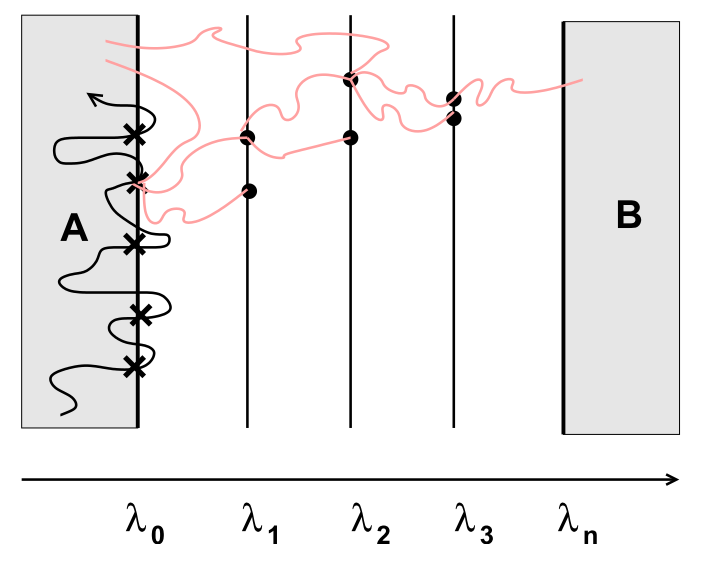
\includegraphics[width=0.8\linewidth]{Figures/FFS.jpg}
  \caption{Nog maken}
\end{figure}

